% Options for packages loaded elsewhere
\PassOptionsToPackage{unicode}{hyperref}
\PassOptionsToPackage{hyphens}{url}
\documentclass[
  ignorenonframetext,
]{beamer}
\newif\ifbibliography
\usepackage{pgfpages}
\setbeamertemplate{caption}[numbered]
\setbeamertemplate{caption label separator}{: }
\setbeamercolor{caption name}{fg=normal text.fg}
\beamertemplatenavigationsymbolsempty
% remove section numbering
\setbeamertemplate{part page}{
  \centering
  \begin{beamercolorbox}[sep=16pt,center]{part title}
    \usebeamerfont{part title}\insertpart\par
  \end{beamercolorbox}
}
\setbeamertemplate{section page}{
  \centering
  \begin{beamercolorbox}[sep=12pt,center]{section title}
    \usebeamerfont{section title}\insertsection\par
  \end{beamercolorbox}
}
\setbeamertemplate{subsection page}{
  \centering
  \begin{beamercolorbox}[sep=8pt,center]{subsection title}
    \usebeamerfont{subsection title}\insertsubsection\par
  \end{beamercolorbox}
}
% Prevent slide breaks in the middle of a paragraph
\widowpenalties 1 10000
\raggedbottom
\AtBeginPart{
  \frame{\partpage}
}
\AtBeginSection{
  \ifbibliography
  \else
    \frame{\sectionpage}
  \fi
}
\AtBeginSubsection{
  \frame{\subsectionpage}
}
\usepackage{iftex}
\ifPDFTeX
  \usepackage[T1]{fontenc}
  \usepackage[utf8]{inputenc}
  \usepackage{textcomp} % provide euro and other symbols
\else % if luatex or xetex
  \usepackage{unicode-math} % this also loads fontspec
  \defaultfontfeatures{Scale=MatchLowercase}
  \defaultfontfeatures[\rmfamily]{Ligatures=TeX,Scale=1}
\fi
\usepackage{lmodern}
\ifPDFTeX\else
  % xetex/luatex font selection
\fi
% Use upquote if available, for straight quotes in verbatim environments
\IfFileExists{upquote.sty}{\usepackage{upquote}}{}
\IfFileExists{microtype.sty}{% use microtype if available
  \usepackage[]{microtype}
  \UseMicrotypeSet[protrusion]{basicmath} % disable protrusion for tt fonts
}{}
\makeatletter
\@ifundefined{KOMAClassName}{% if non-KOMA class
  \IfFileExists{parskip.sty}{%
    \usepackage{parskip}
  }{% else
    \setlength{\parindent}{0pt}
    \setlength{\parskip}{6pt plus 2pt minus 1pt}}
}{% if KOMA class
  \KOMAoptions{parskip=half}}
\makeatother
\usepackage{graphicx}
\makeatletter
\newsavebox\pandoc@box
\newcommand*\pandocbounded[1]{% scales image to fit in text height/width
  \sbox\pandoc@box{#1}%
  \Gscale@div\@tempa{\textheight}{\dimexpr\ht\pandoc@box+\dp\pandoc@box\relax}%
  \Gscale@div\@tempb{\linewidth}{\wd\pandoc@box}%
  \ifdim\@tempb\p@<\@tempa\p@\let\@tempa\@tempb\fi% select the smaller of both
  \ifdim\@tempa\p@<\p@\scalebox{\@tempa}{\usebox\pandoc@box}%
  \else\usebox{\pandoc@box}%
  \fi%
}
% Set default figure placement to htbp
\def\fps@figure{htbp}
\makeatother
\setlength{\emergencystretch}{3em} % prevent overfull lines
\providecommand{\tightlist}{%
  \setlength{\itemsep}{0pt}\setlength{\parskip}{0pt}}
\usepackage{bookmark}
\IfFileExists{xurl.sty}{\usepackage{xurl}}{} % add URL line breaks if available
\urlstyle{same}
\hypersetup{
  hidelinks,
  pdfcreator={LaTeX via pandoc}}

\author{\texorpdfstring{}{}}
\date{}

\begin{document}

\begin{frame}{Gresham's Law and the Fracture of Mythopoetic Alchemy}
\protect\phantomsection\label{greshams-law-and-the-fracture-of-mythopoetic-alchemy}
When international silver values fluctuated against the enforced
Newtonian mint ratio of 1717, they triggered the mechanical arbitrage of
Gresham's Law: ``bad money drives out good'' {[}@thornton1802nature{]}.
Because gold was systematically overvalued within the English
Channel---Newton's guinea priced at 21 shillings domestically while
equivalent gold commanded only 20s 9d in Spain or Portugal---bullion
merchants melted full-weight silver coins and shipped the raw bullion to
France, India, and China, where its elemental weight commanded
significantly higher purchasing power {[}@quinn1996competing{]}. An
engineered mathematical disparity hollowed out the domestic money
supply.

\begin{block}{Velde's Mathematical Formalization of Transatlantic
Bimetallic Instability}
\protect\phantomsection\label{veldes-mathematical-formalization-of-transatlantic-bimetallic-instability}
To formalize this entropic decay, modern economic historians such as
François Velde define the bimetallic equilibrium via the relationship
between the statutory Mint Ratio (\(M\)) and the global commodity Market
Ratio (\(R\)), bounded by transaction and melting costs (\(c\))
{[}@velde2005bimetallism{]}. The condition for a functional, meta-stable
bimetallic circulation is expressed mathematically as:

\begin{equation}
\label{eq:bimetallic_bounds}
M - c < R < M + c
\end{equation}

When the international market ratio of silver to gold climbs beyond the
domestic limit erected by the state (\(R > M + c\)), silver becomes
undervalued at the mint. Arbitrageurs mathematically optimize their
portfolios by melting down full-weight silver coins---the ``Lunar
Flux''---and exporting the bullion to France, India, or the Far East,
where its elemental weight commands a higher purchasing power. The East
India Company played a central role in this drainage, trading English
silver in Asia where it commanded premium value amid regional gold
scarcity; by 1730, these asymmetric flows had delivered 15.5 tonnes of
gold into the Bank of England's vaults while emptying the kingdom of
circulating silver {[}@quinn2007recoinage{]}. This arbitrage drained the
physical economy of its circulating medium, leaving behind only clipped,
worn, or counterfeit silver, alongside the static, hoarded gold.
\end{block}

\begin{block}{Del Mar's Historiographic Reading of the Bimetallic
Marriage}
\protect\phantomsection\label{del-mars-historiographic-reading-of-the-bimetallic-marriage}
However, analyzing this financial collapse exclusively through
quantitative arithmetic obscures its ontological
implications---implications that William Blake recognized implicitly.
The 19th-century monetary historian Alexander Del Mar later framed this
dual-standard through a structural lens that resonates with Blakean
mythology. In his historiographies of money, Del Mar casts monetary
equilibrium not as a natural fact of intrinsic metallic value, but as an
artifact of state numerary authority---a socio-political synthesis where
circulating tokens maintain equilibrium in the monetary firmament under
the sovereign prerogative of the state {[}@delmar1895history{]}.
Analyzing money as a legal and numerical mechanism rather than a pure
commodity unmasks the bimetallic pairing as a representation of
sovereign decree rather than intrinsic divine right. Marc Flandreau
extends this historiography, characterizing classical bimetallism as a
form of economic alchemy conjuring stabilizing stasis from the
metaphysical chaos of global trade by binding two independent metallic
volatilities into a single legal fiction
{[}@flandreau1996bimetallism{]}.
\end{block}

\begin{block}{The Thermodynamic Decay from Bimetallic Generation to
Monometallic Ulro}
\protect\phantomsection\label{the-thermodynamic-decay-from-bimetallic-generation-to-monometallic-ulro}
London's legally entrenched overvaluation of gold severed this
alchemical harmony {[}@quinn1996competing{]}. Bimetallism was,
inherently, a \emph{Twofold Generative} tension (see the Fourfold
Vision): an unstable but vitalizing socio-economic synthesis of the
Solar (Gold/Love/Authority) and the Lunar (Silver/Wisdom/Circulation).
The bullion merchants---driven by the atomizing, Epicurean
\emph{clinamen} of profit and private self-interest---melted down the
lunar element to hoard the solar. That rapacity maps onto the
Erdman-Urizen reading of empire and war finance established in our
Introduction {[}@erdman1954prophet{]}.

For Blake, this is the very definition of the state of \emph{Generation}
decaying into \emph{Ulro} (the void). Production and exchange were no
longer aimed at sustaining human community or fulfilling human needs,
but were captured by the paper-led churn of arbitrage. In
\emph{Jerusalem} Plate 27 Blake names the fixing of labour and the
invention of ``allegoric riches'' (see
\hyperlink{sec-allegoric-riches}{§ The fixing of labour and allegoric
riches}) {[}@erdman1988complete; @sklar2011blake{]}---precisely the
moment when the living economy of human exchange is seized by the
arithmetic of financial extraction. The bimetallic synthesis fractured
under Gresham friction because it was a catastrophic clash between
living, dual commodity interaction and the dead, reductionist geometry
of the fixed Mint Ratio. Single Vision attempted, and failed, to bind
generative duality. This drove the entire system toward monometallic
isolation (as detailed in the discussion of the 1816 Coinage Act).
Gresham's law, in this mythopoetic register, is not merely a law of
economics, but a law of spiritual thermodynamics: the inevitable
degradation of meaning when human relationships are mediated exclusively
by rigid, monistic metrics.

\begin{figure}
\centering
\pandocbounded{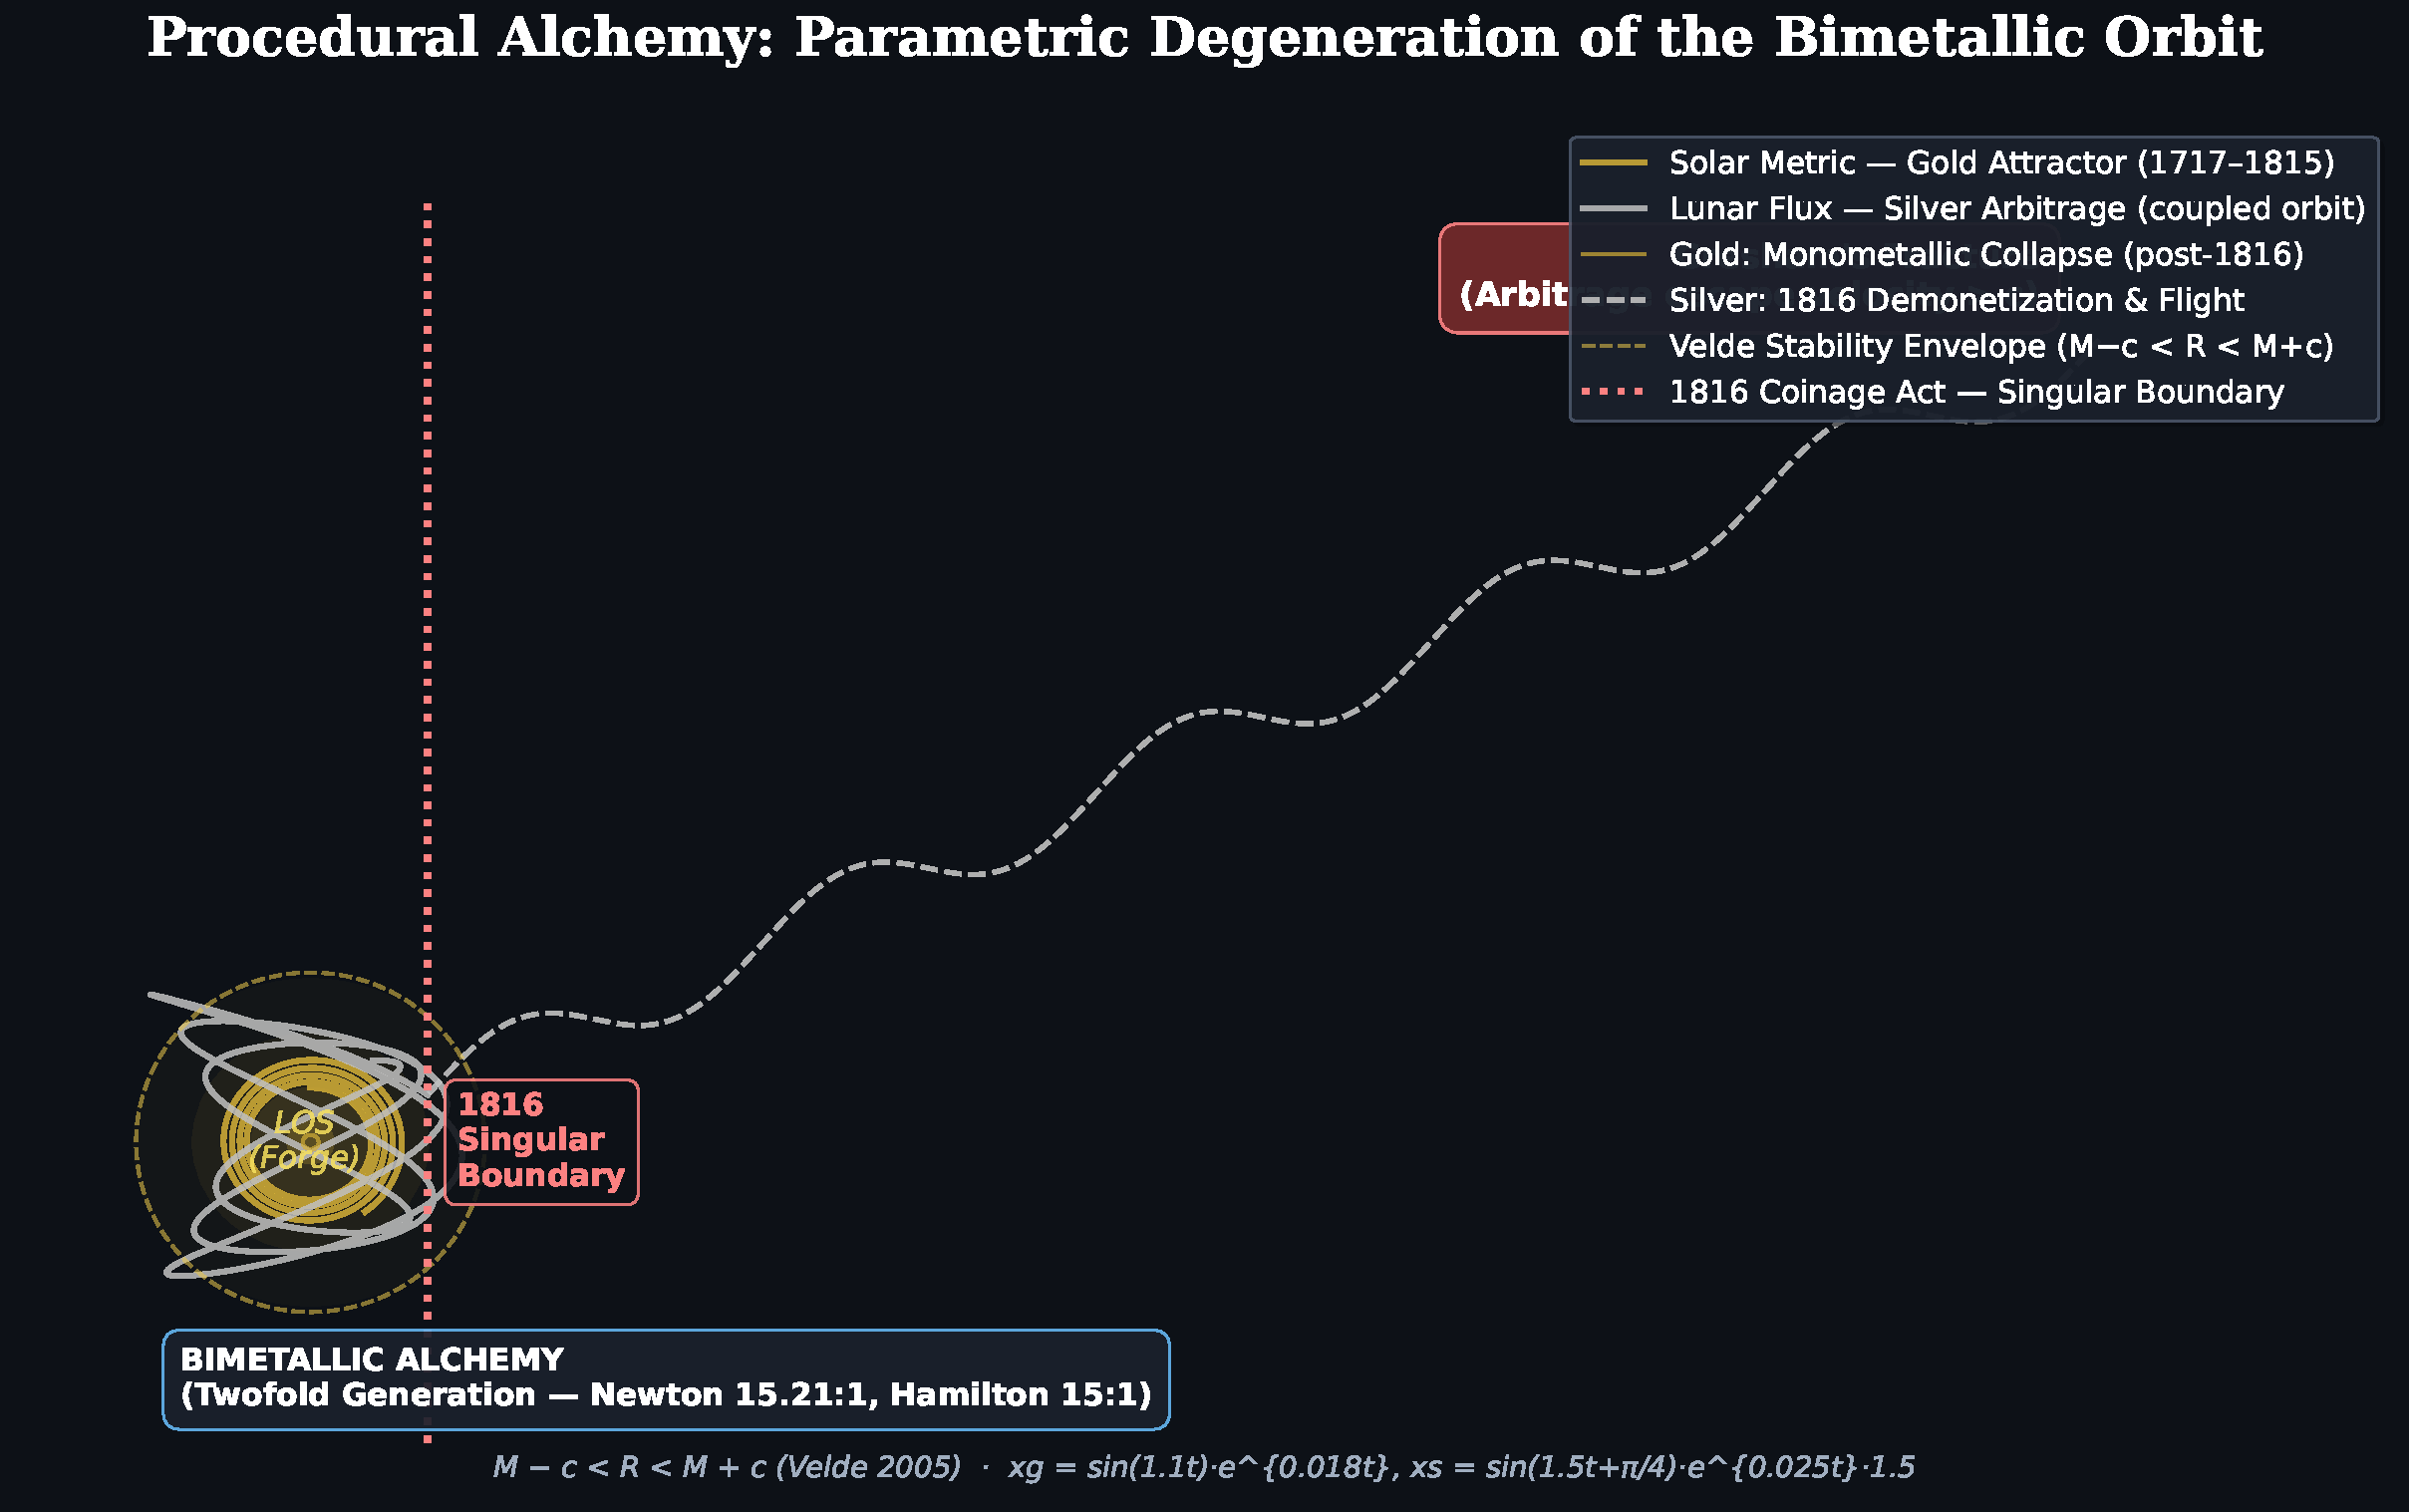
\includegraphics[keepaspectratio,alt={Procedural Alchemy of Bimetallic Vectors --- Parametric Degeneration of Bimetallic Orbit. This procedurally generated 5000-point Harmonograph maps the historical vectors of Solar Gold (the central, tight attractor) and Lunar Silver (the wider, sweeping orbit of the 1.5 ratio) locked in meta-stable Twofold Generation. Mathematical harmony holds until the Velde stability ellipse threshold is breached (R \textgreater{} M + c). At the 1816 singular boundary, Gresham's arbitrage escape velocity is crossed: the Solar Gold vector collapses inward to a static geometric dot at the Urizen pole (Single Vision / The Gold Standard with 4-layer glow rings), while the Lunar Silver vector violently breaks orbit toward the Los pole, escaping tangentially into chaotic space---modeling the physical demonetization of silver under the Coinage Act (56 Geo. III c.68) and the total eradication of the bimetallic generative synthesis. Includes the parametric equation xg = \textbackslash sin(1.1t)e\^{}\{0.018t\}, xs = \textbackslash sin(1.5t+\textbackslash pi/4)e\^{}\{0.025t\} \textbackslash cdot 1.5.}]{../figures/alchemical_bimetallism_dark.pdf}}
\caption{Procedural Alchemy of Bimetallic Vectors --- Parametric
Degeneration of Bimetallic Orbit. This procedurally generated 5000-point
Harmonograph maps the historical vectors of Solar Gold (the central,
tight attractor) and Lunar Silver (the wider, sweeping orbit of the 1.5
ratio) locked in meta-stable Twofold Generation. Mathematical harmony
holds until the Velde stability ellipse threshold is breached
(\(R > M + c\)). At the 1816 singular boundary, Gresham's arbitrage
escape velocity is crossed: the Solar Gold vector collapses inward to a
static geometric dot at the Urizen pole (Single Vision / The Gold
Standard with 4-layer glow rings), while the Lunar Silver vector
violently breaks orbit toward the Los pole, escaping tangentially into
chaotic space---modeling the physical demonetization of silver under the
Coinage Act (56 Geo. III c.68) and the total eradication of the
bimetallic generative synthesis. Includes the parametric equation
\(xg = \sin(1.1t)e^{0.018t}, xs = \sin(1.5t+\pi/4)e^{0.025t} \cdot 1.5\).}\label{fig-alchemy}
\end{figure}
\end{block}
\end{frame}

\end{document}
